\chapter{Results}

The predictions of the previous sections are tested on \emph{trans}-polyacetylene. Therefore the convergence is checked first. Since \emph{trans}-polyacetylene has an alternation of single and double bonds between the carbon atoms, a unit cell containing two CH-groups with periodic boundary conditions in one dimension is used (see \cref{image_scheme_polyacetylene_unit_cell}). 

\section{Convergence Testing of Polyacetylene}
\begin{figure}[!b]
	\centering
	\begin{tikzpicture}[show background rectangle, scale = 0.8]
	\foreach \x in {0,4,...,8}{
		\foreach \y in {-1, 1}{
			\node [circle, draw] at (\x + 0.8*\y, \y) {C};
			\node [circle, draw] at (\x + 0.8*\y, 2 * \y) {H};
	}}
	\draw (2.2, 3) -- (2, 3) -- (2,-3) -- (2.2, -3);
	\draw (5.8, 3) -- (6, 3) -- (6,-3) -- (5.8, -3);
	\draw [dotted, line width = 1.5] (-2,0) -- (-1.5,0);
	\draw [dotted, line width = 1.5] (9.5, 0) -- (10,0);
	\end{tikzpicture}
	\caption{Scheme: Unit cell for \emph{trans}-polyacetylene with periodic boundary conditions in one dimension}
	\label{image_scheme_polyacetylene_unit_cell}
\end{figure}
\begin{figure}[!p]
	\centering
	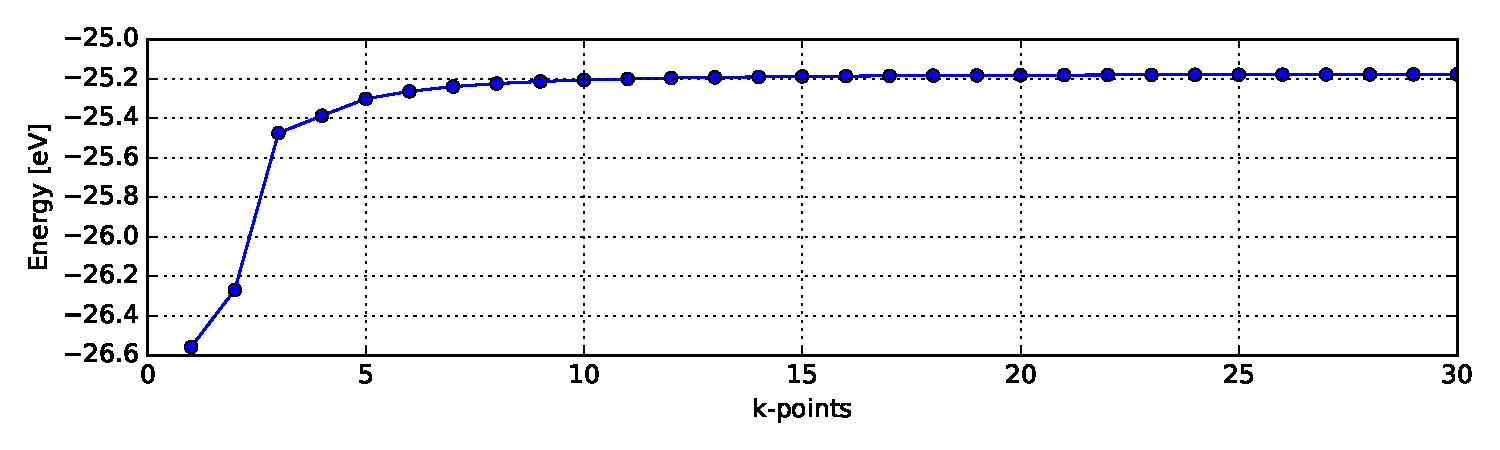
\includegraphics[width = 11cm]{Images/polyacetylene/convergence/kpts-energy}
	\caption{Ground state energy of relaxed polyacetylene in respect to the number of $k$-points}
	\label{image_poly_kpts_energy}
\end{figure}
\begin{figure}[!p]
	\centering
	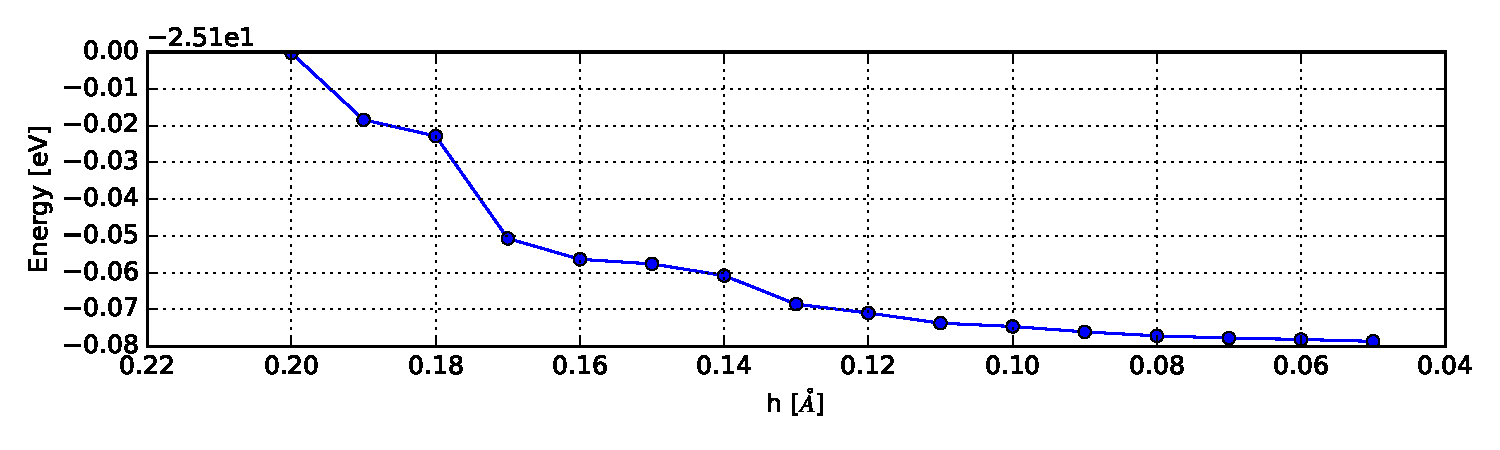
\includegraphics[width = 11cm]{Images/polyacetylene/convergence/gridspacing-energy}
	\caption{Ground state energy of relaxed polyacetylene in respect to the grid spacing}
	\label{image_poly_grid_energy}
\end{figure}
\begin{figure}[!p]
	\centering
	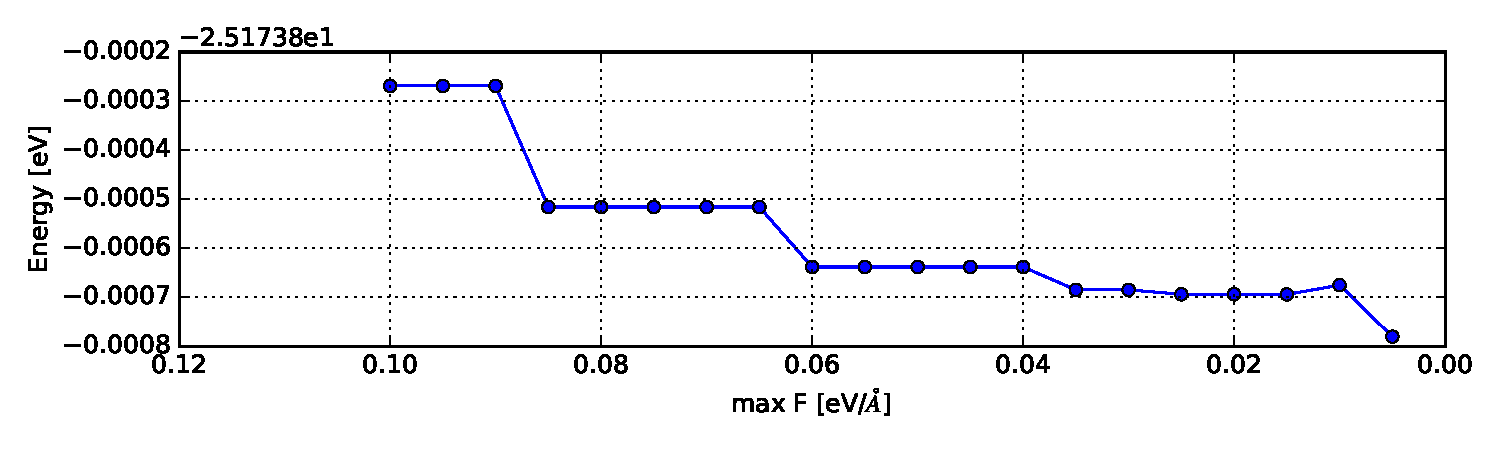
\includegraphics[width = 11cm]{Images/polyacetylene/convergence/forces-energy}
	\caption{Ground state energy of relaxed polyacetylene in respect to the maximum force, for which the relaxation process stops}
	\label{image_poly_force_energy}
\end{figure}
\begin{figure}[!p]
	\centering
	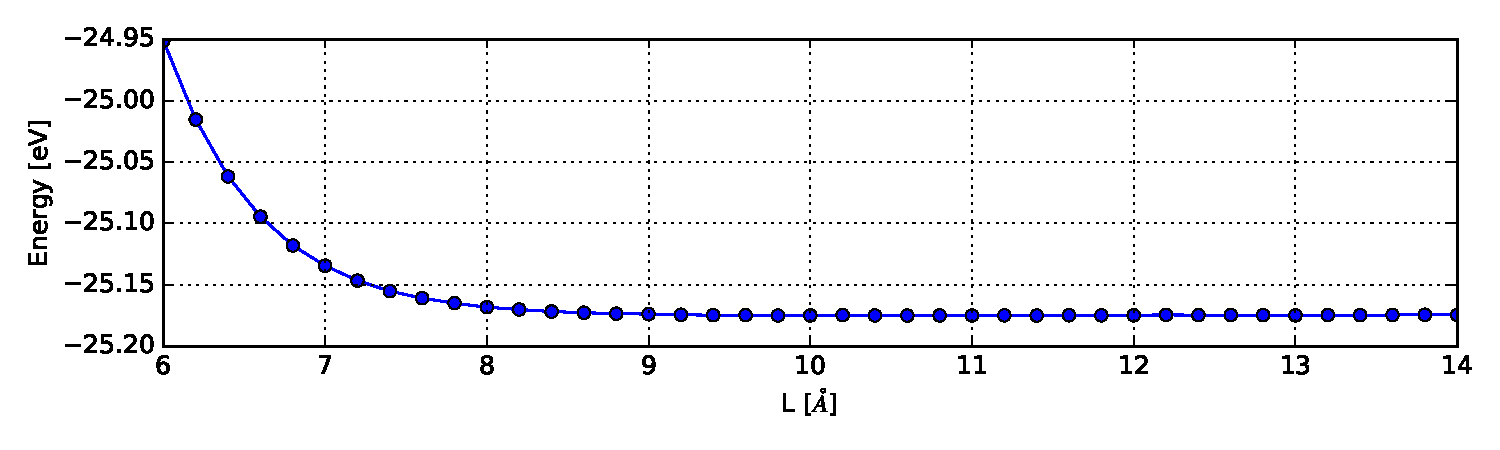
\includegraphics[width = 11cm]{Images/polyacetylene/convergence/unit_cell_width}
	\caption{Ground state energy of relaxed polyacetylene in respect to width of the unit cell (not in direction of periodic boundary condition)}
	\label{image_poly_width_energy}
\end{figure}
To check the convergence in respect to a certain parameter, all other parameters are chosen in a way, that the energy is definitely converged in respect to them. This includes also a relaxation of the atom positions in each step.\\
First the convergence of the ground state energy in respect to the number of used $k$- points is tested, whereat automatic \textsc{Brillouin} zone sampling is used. It can be seen, that the energy is quite good converged for approximately 15 $k$-points (see \cref{image_poly_kpts_energy}), since a comparison of the energies for $15$ and $100$ $k$-points leads to a difference of only $\unit[0.014]{eV}$.\\
In \cref{image_poly_grid_energy} the ground state energy in respect to the grid spacing can be seen. Since the number of grid points grows with $\nicefrac{1}{h^3}$, it is very important to find a reasonable compromise between computing time and accuracy. Because our system isn't that big, a $h$ value of $\unit[0.1]{\AA}$ is used for further calculations.\\
The lowering of the ground state energy in respect to the maximum force for the relaxation process of the cores is in comparison with previous dependencies small. Therefore a maximum force of $\unitfrac[0.1]{eV}{\AA}$ should be appropriate.\\
Finally the convergence of the energy in respect to the unit cell width (not in the direction of the periodic boundary condition) is tested. As can be seen in \cref{image_poly_width_energy}, the ground state energy increases for small unit cell widths, what can be understood intuitively by comparison to the quantum mechanical 'particle in a box'. For a with of approximately $\unit[9]{\AA}$ a stable level is reached, what corresponds with a minimal distance between core and cell surface of approximately $\unit[3]{\AA}$.



\section{Real Stuff}

In the following plots the $k$-point values are always given relative to the basis vectors of the reciprocal unit cell. Thus a value of $k = \pm 0.5$ corresponds to a state at the edge of the \textsc{Brillouin} zone.
\chapter{Chaos}
To model the charging applied with CDFT of the two regions with $\pm q$ two approaches will be tested:
\begin{compactitem}
	\item[1)] simple modifications of the wave functions under the assumption that all $k$-points contribute equally to the charge displacement
	\item[2)] modification of the Hamiltonian describing the external potential for the different regions
\end{compactitem}
The first approach leads to the valence wave function:
\begin{align}
\Psi_k^{(v)}(q) &= \sqrt{\frac{1}{2}-\frac{q}{2}}c_k^{\dagger(e)}- \sqrt{\frac{1}{2}+\frac{q}{2}}\frac{\epsilon_k - i \Delta_k}{|E_k|}c_{k}^{\dagger(o)}
\end{align}
with the following expectation values for the energies:
\begin{align}
\left\langle\Psi_k^{(v)}(q)\Big|\mathcal{H}_{k}\Big|\Psi_k^{(v)}(q)\right\rangle &= -\sqrt{1-q^2} |E_k|
\end{align}
And the sum over the HOMO-band energies:
\begin{align}
E_0(q) &= -\frac{4Nt_0}{\pi} \sqrt{1-q^2}
\label{equation_equal_charge}
\end{align}
The second approach leads to the Hamiltonian which decreases/increases the energies at the even/odd positions:
\begin{align}
	\mathcal{H}_k &= \left[\epsilon_k + i\Delta_k\right]c_{k}^{\dagger(e)}c_{k}^{(o)} + \left[\epsilon_k-i\Delta_k \right]	c_{k}^{\dagger(o)}c_{k}^{(e)} - V n^{(e)}_k + V n^{(o)}_k
\end{align}
or in matrix notation:
\begin{align}
	\mathcal{H}_k &= \begin{pmatrix*}[c]
	-V & \epsilon_k + i \Delta_k \\
	\epsilon_k - i \Delta_k & V
	\end{pmatrix*}
\end{align}
with the eigenvalues $E_k = \pm \sqrt{V^2+\epsilon_k^2+\Delta_k^2}$ and the eigenstates\footnote{the valence state corresponds with the lower signs}:
\begin{align}
	\vv{\Psi}_k(V) &= \left[2\left(E_k^2\mp V|E_k|\right)\right]^{\nicefrac{-1}{2}} \cdot \begin{pmatrix*}[c]
	-V\pm \sqrt{V^2+\epsilon_k^2+\Delta_k^2}\\
	\epsilon_k - i \Delta_k
	\end{pmatrix*}
\end{align}
For $V=0$ this matches the previous result. 
The sum over the HOMO-band energies becomes approximately:
\begin{align}
	E_0 &= \frac{-2N}{\pi} \sqrt{V^2+4t_0^2}
	\label{equation_ext_pot}
\end{align} 
Since a bigger absolute of the displaced charge $\left|q\right|$ is expected for a bigger absolute of the external potential $\left|V\right|$ these two approaches contradict each other (compare \cref{equation_equal_charge,equation_ext_pot}).

\section{Other Preparations}
\begin{figure}[!h]
\centering
\begin{tikzpicture}[show background rectangle, scale = 1]
\foreach \x in {0,...,7}{
	\draw[line width=2pt] (\x,0) .. controls (\x + 1, 2) and (\x - 1 , 2) .. cycle .. controls (\x + 1, -2) and (\x - 1 , -2) .. cycle;
}
\foreach \x in {0, 4}
	\foreach \y in {0, 1}
		\foreach \z in {-1, 1}
		\node at (\x + \y - \z + 1, \z) {\huge +};
\foreach \x in {0, 4}{
	\foreach \y in {0, 1}{
		\foreach \z in {-1, 1}{
			\node at (\x + \y - \z + 1, -\z) {\huge -};
}}}
\draw[line width = 0.2] (-0.1, -1.8) -- +(-0.3, 0) -- +(-0.3 ,3.6) -- +(0,3.6);
\draw[line width = 0.2] (1.1, -1.8) -- +(0.3, 0) -- +(0.3 ,3.6) -- +(0,3.6);
\draw[line width = 0.2] (3.9, -1.8) -- +(-0.3, 0) -- +(-0.3 ,3.6) -- +(0,3.6);
\draw[line width = 0.2] (7.1, -1.8) -- +(0.3, 0) -- +(0.3 ,3.6) -- +(0,3.6);
\end{tikzpicture}
\end{figure}




\section{Hydrogen Chain}

A simple system of equidistant hydrogen atoms is used to test the predictions of the earlier motivated Hamiltonian. For this purpose the set-up and convergence of the unit cell will be tested. Afterwards the results from the application of CDFT to the band structure will be shown and compared to the predictions of our modeling approaches.

\subsection{Unit Cell Set-Up}
Even if there's no distortion, a unit cell with two hydrogen atoms is needed, because later the application of the external potential and the consequential charge displacement will break the symmetry. All calculations for hydrogen will be performed using spin polarization, since this lowers the ground state energy and later this will be essential for the convergence of the wave functions (\textbf{WRONG}) in the presence of the external potentials. Therefore it's necessary for the optimizer to break the symmetry by setting the initial magnetic moments of the atoms to $\pm\nicefrac{1}{2}$. 


\subsection{Results}

First of all the HOMO band shows the expected $E(k)\propto -\cos(ka)$ behaviour (see \cref{image_hydrogen_bandstructure}). Through fitting to the HOMO band the hopping parameter $t_0 = \unit[4.78]{eV}$ can be obtained.

\begin{figure}[!bth]
	\centering
	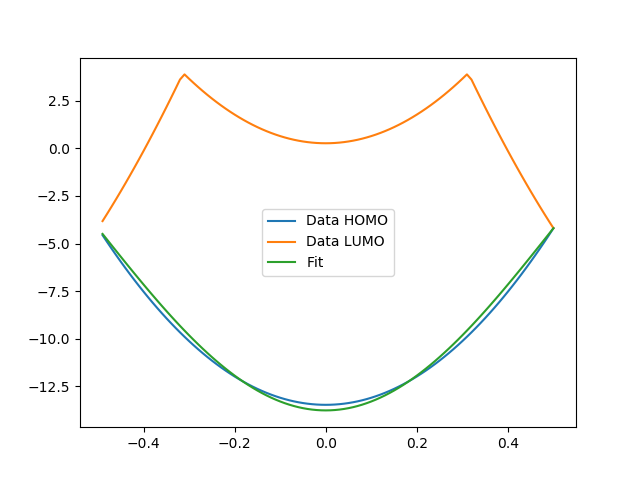
\includegraphics[width = 10cm]{Images/Hydrogen/hydrogen_bandstructure}
	\caption{$E(k)$}
	\label{image_hydrogen_bandstructure}
\end{figure}

In the next step the band structures for the periodically charged hydrogen atoms will be calculated (see \cref{image_hydrogen_charged_bands}). As expected from the symmetry the band structures do not depend on the direction (sign) of the charge displacement. It can also be seen, that the influence of charging is bigger for $k$-points closer to the edge of the Brillouin zone and the bands become shifted to lower energies. Both is in good agreement with the predictions of the Hamiltonian.

\begin{figure}
	\centering
	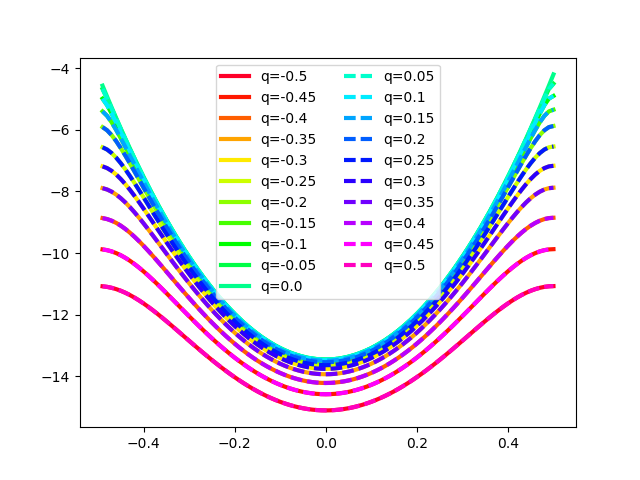
\includegraphics[width = 12cm]{Images/Hydrogen/hydrogen_charged_bands}
	\caption{$E(k, q)$}
	\label{image_hydrogen_charged_bands}
\end{figure}




In \cref{image_hydrogen_charge_potential} the height of the Gaussian potentials causing the charge displacement as a function of the transferred charge is shown. Again the symmetry is as expected and in the region of $-0.2 \le q \le 0.2$ the dependency is approximately linear.

\begin{figure}
	\centering
	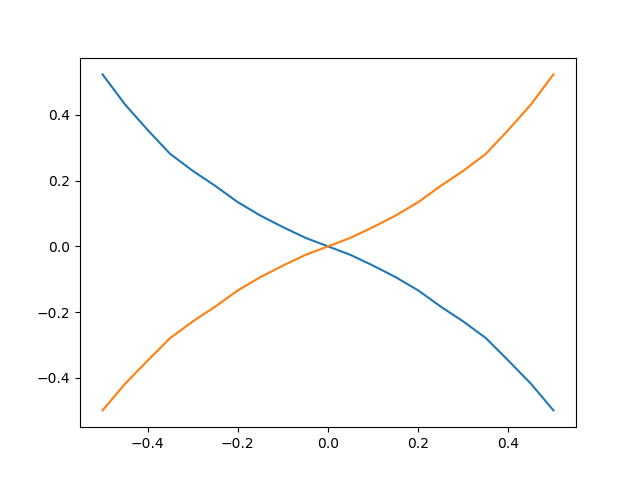
\includegraphics[width = 10cm]{Images/Hydrogen/hydrogen_charge_potential}
	\caption{$V(q)$}
	\label{image_hydrogen_charge_potential}
\end{figure}

From the model Hamiltonian the state energy at the edge of the Brillouin zone ($k\cdot a = \nicefrac{\pi}{2}$) is expected to have the form $E_\text{edge} = -\sqrt{V^2} = -\sqrt{c^2\cdot U_\text{CDFT}^2}$. As can be seen in \cref{image_hydrogen_border_energy_potential} this matches the results of the simulation very well. From a fit to this data the ratio between the theoretical potential and the voltage from CDFT can be obtained: $V \approx \unit[13.265]{e} \cdot U_\text{CDFT}$.

\begin{figure}
	\centering
	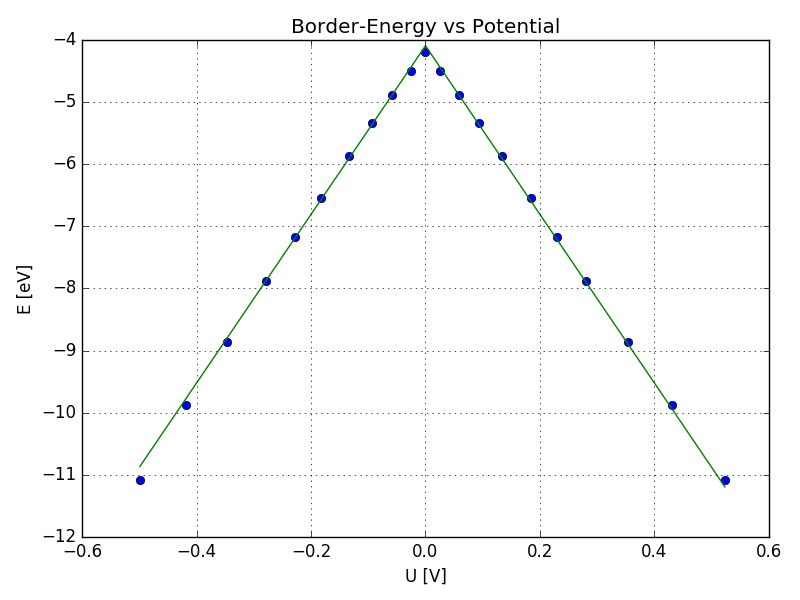
\includegraphics[width = 12cm]{Images/Hydrogen/hydrogen_border_energy}
	\caption{$E(U)$}
	\label{image_hydrogen_border_energy_potential}
\end{figure}

Analogously this ratio can be calculated by fitting the energy at the gamma point to \linebreak $E_\text{gamma} = -\sqrt{c^2 \cdot U_\text{CDFT}^2 + 4 \cdot t_0^2}$ (see \cref{image_hydrogen_mid_energy_potential}). Here the proportionality constant becomes $V \approx \unit[11.289]{e} \cdot U_\text{CDFT}$, which corresponds to a relative difference of approximately 20\%. To take a closer look at this effect the proportionality constant is calculated by fitting for many different $k$-points (see \cref{image_hydrogen_proportionality_constant}). 
\begin{figure}
	\centering
	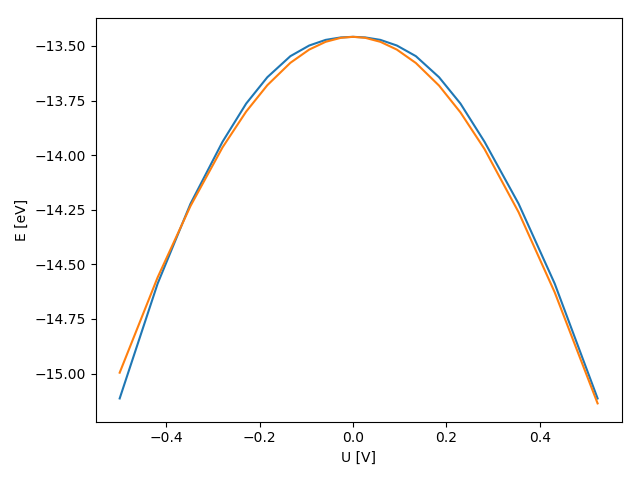
\includegraphics[width = 12cm]{Images/Hydrogen/hydrogen_mid_energy}
	\caption{$E(U)$}
	\label{image_hydrogen_mid_energy_potential}
\end{figure}

\begin{figure}
	\centering
	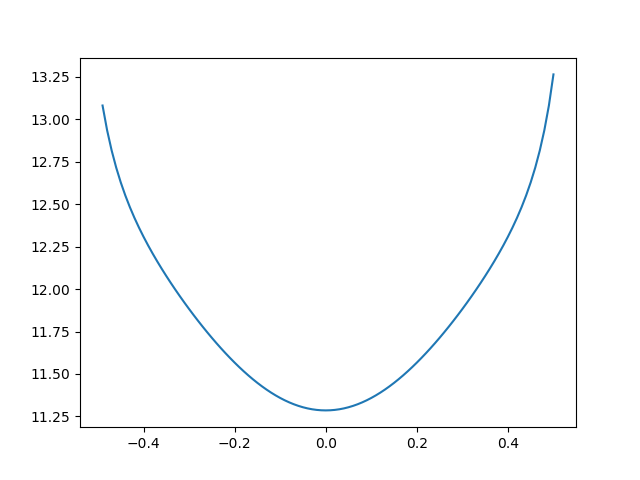
\includegraphics[width = 12cm]{Images/Hydrogen/hydrogen_c_k_dependency}
	\caption{$c(k)$}
	\label{image_hydrogen_proportionality_constant}
\end{figure}